\graphicspath{{content/2_design/figures/}}
\section{Digital Motor Controller: Switch and Current Sensor}

\subsection{Configuration}

The low-side switch will be a FQD13N06L NMOS transistor driven by the ESP using PWM. This transistor was chosen due to its
low turn-on voltage, eliminating the need for any gain circuitry. A resistor will be used in series from the ESP to the MOSFET to
prevent surge currents due to the capacitive nature of the MOSFET gate. A pull-down resistor will also be used to ensure
the circuit is fully off when the ESP pin is in a high impedance state (e.g. when the circuit is powered down or during startup).

The current sensor circuit will also be a non-inverting amplifier with a filter, similar to the circuit used for the analog wheel,
however care needs to be taken to ensure the PWM signal is filtered adequately. The sense resistor will be placed on the low side
of the MOSFET to avoid the use of a differential amplifier.

\subsection{Input Resistors}

In order to calculate $R_a$, the series input resistor from the ESP, the assumption is made that the series resistance before the equivalent gate capacitance is zero.
Since the current equation for an RC circuit is $I(t) = I_0 e^{-t/\tau}$, with $I_0 = \frac{V}{R}$, the surge current will be $I_0$ at $t = 0$. Choose $I_0 = \SI{10}{mA}$
$\therefore R_a = \frac{V_{cc}}{I_0} = \frac{\SI{3.3}{V}}{\SI{10}{mA}} = \SI{330}{\ohm}$.

The pull-down resistor should be chosen so that the ESP is not loaded during operation, thereby affecting the voltage. If it is chosen that this resistor consumes
maximum additional current of $\SI{100}{\micro\ampere}$, the resistor should then be $R_{b(min)} = \frac{\SI{3.3}{V}}{\SI{100}{\micro\ampere}} = \SI{33}{\kilo\ohm}$.
Choose $R_b = \SI{100}{\kilo\ohm}$.

\subsection{Transistor Requirements}

It should be checked that the FQD13N06L transistor is suitable with regards to turn-on voltage, current capabilities, and series resistance.
\begin{itemize}
    \item The $V_{gs}$ threshold voltage should be checked to ensure the transistor is turned on fully. According to \cite{datasheetFQD13N06L},
          the maximum turn-on voltage of the transistor is 2.5 V. Since the ESP will output a 3.3 V PWM signal on its digital pins,
          the transistor will be turned on fully since the pin's output voltage is 32\% higher than the required $V_{gs}$ threshold.
    \item The current requirements should be compared with the transistor's current capabilities. A maximum stall current of 750 mA is required.
          If the transistor is not capable of handling this, it might be damaged due to excess heat dissipation. Choose $I_{max} = \SI{1}{A}$ for additional headroom.
          Again, according to \cite{datasheetFQD13N06L}, the transistor can handle a continuous current of $\SI{7}{A}$ with its case kept at \SI{100}{\celsius}. This is well
          within the current limitation of the motor.
    \item The equivalent series resistance of the transistor should be analyzed at different forward currents in order to determine the voltage drop it will cause
          in series with the motor. The datasheet reveals that, at $V_{gs} = \SI{5}{V}$, the forward resistance only varies from around $\SI{110}{\milli\ohm}$ to $\SI{120}{\milli\ohm}$
          as current increases to 10 A. At currents of around 1 A, a maximum voltage drop of around 0.12 V will be found, which is negligible and means that the motor will receive almost the
          full 7.2 V. This is also at maximum current - at lower current levels, the voltage drop will be even less, however in this design this will be slightly countered by the fact that
          $V_{gs} = \SI{3.3}{V}$.
\end{itemize}

\subsection{Current Sensor}

The same design as in \ref{design_currentSensor} will be used. Since a PWM frequency of 20 kHz will be used, the current sensor filtering frequency,
which is designed to adequately filter out a 1 kHz signal, is more than adequate, and will filter out the fundamental frequency and all harmonics.
The frequency could even be raised, however will be kept the same in order to match it with the analog wheel current sensor.

The rest of the design of the sensor can also be kept identical due to the final receiver of the value (the ESP) being the same. These design decisions, as well as the justifications
to keep them, are documented below:
\begin{itemize}
    \item The non-inverting gain will be 825, which allows for current values of up to 400 mA to be read.
    \item The filter cutoff frequency will remain at 11 Hz to have a slower response which heavily filters out any noise.
    \item A 3.3 V supply will be used to limit the output and prevent damaging the ESP's input pins.
\end{itemize}

\subsection{Circuit Diagram}

\begin{figure}[!htb]
  \centering
  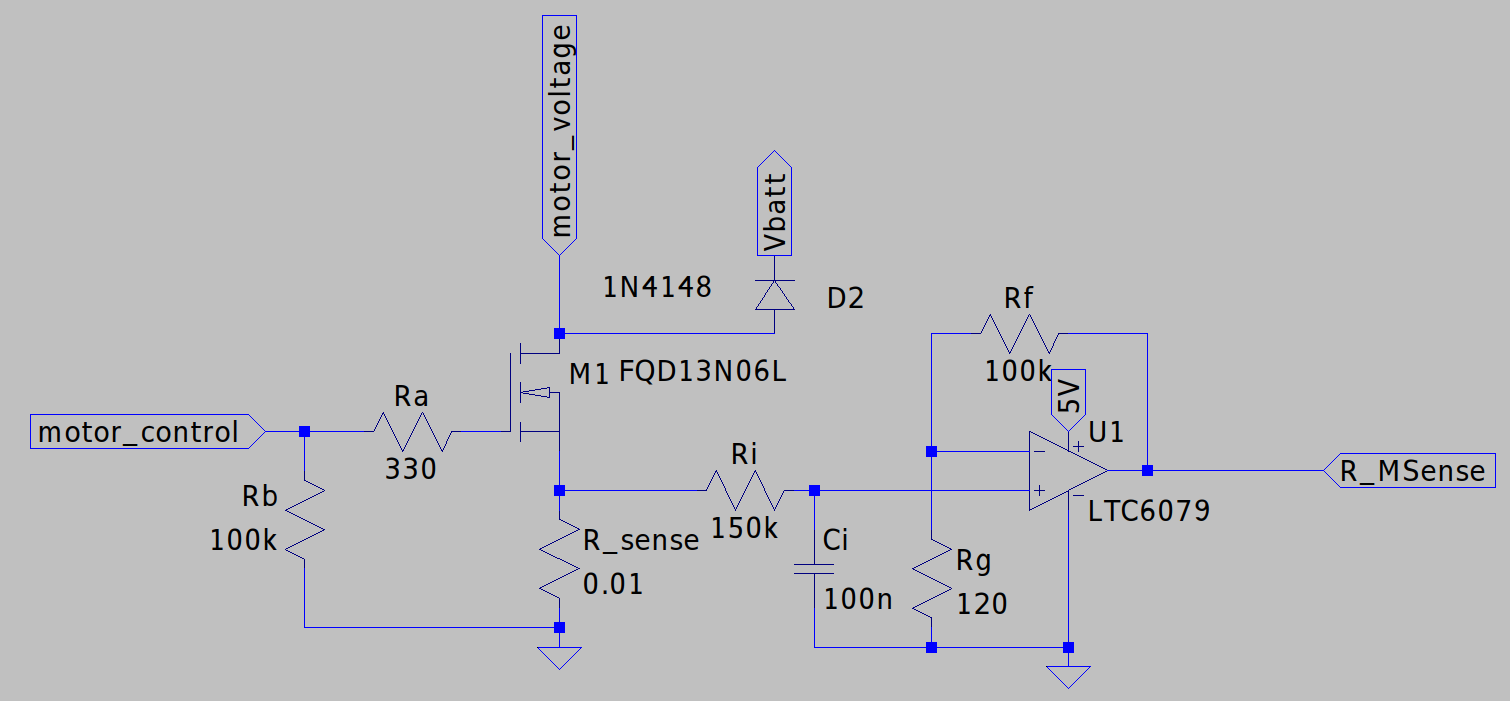
\includegraphics[width=0.7\textwidth]{digitalMotorController_circuitDiagram}
  \caption{Digital Motor Controller and Current Sensor Circuit Diagram}
  \label{fig:digitalMotorController_circuitDiagram}
\end{figure}